\documentclass[lettersize,journal]{IEEEtran}
%\documentclass[conference]{IEEEtran}
\usepackage{amsmath,amsfonts}
\usepackage{algorithmicx}
\usepackage{algorithm}
\usepackage{array}
\usepackage[caption,font=normalsize,labelfont=sf,textfont=sf]{subfig}
\usepackage{textcomp}
\usepackage{stfloats}
\usepackage{url}
\usepackage{verbatim}
\usepackage{graphicx}
\usepackage{cite}
\usepackage{tabularx}
%\documentclass[a4paper, 10pt, conference]{ieeeconf}   
%\usepackage{blindtext, graphicx}
%\usepackage{listings}
%\lstset { %
%	language=C++,
%	numbers=left,
%	breaklines=true,
%	xleftmargin=4em,
%	resetmargins=true,
%	basicstyle=\footnotesize,
%	numberstyle=\footnotesize,
%}
%\usepackage{graphicx}
%\usepackage{amsmath}
%\usepackage{tabularx}
\usepackage[font=normalsize]{caption}

%Pacote para acentos [Por TIAGO]
\usepackage[portuguese]{babel}
%\addto\captionsportuguese{
%	\renewcommand{\figurename}{Figura}
%	\renewcommand{\tablename}{Tabela}
%}
% updated with editorial comments 8/9/2021
\hyphenation{op-tical net-works semi-conduc-tor IEEE-Xplore}

\begin{document}

\title{Confiabilidade de Linhas de Transmissão\\ Utilizando Sistema Sul Brasileiro \\ com 32 Barras}

\author{Leonardo Felipe da Silva dos Santos,~\\ \IEEEmembership{Centro de Excelência em Energia e Sistemas de Potência (CEESP),\\ Programa de Pós-Graduação em Engenharia Elétrica,~\\ Universidade Federal de Santa Maria \\ Santa Maria, Brasil \\ leonardo.santos@acad.ufsm.br}}
        % <-this % stops a space
% \thanks{This paper was produced by the IEEE Publication Technology Group. They are in Piscataway, NJ.}% <-this % stops a space
% \thanks{Manuscript received April 19, 2021; revised August 16, 2021.}}

% The paper headers
% \markboth{Journal of \LaTeX\ Class Files,~Vol.~14, No.~8, August~2021}%
% {Shell \MakeLowercase{\textit{et al.}}: A Sample Article Using IEEEtran.cls for IEEE Journals}

% \IEEEpubid{0000--0000/00\$00.00~\copyright~2021 IEEE}
% Remember, if you use this you must call \IEEEpubidadjcol in the second
% column for its text to clear the IEEEpubid mark.

\maketitle

\begin{abstract}
This document describes the most common article elements and how to use the IEEEtran class with \LaTeX \ to produce files that are suitable for submission to the IEEE.  IEEEtran can produce conference, journal, and technical note (correspondence) papers with a suitable choice of class options. 
\end{abstract}

\begin{IEEEkeywords}
Article submission, IEEE, IEEEtran, journal, \LaTeX, paper, template, typesetting.
\end{IEEEkeywords}

\section{Introdução}
\IEEEPARstart{O}{} sistema elétrico brasileiro é constituído fundamentalmente por usinas hidrelétricas de grande porte, quais essas criam desafios para linhas de transmissão (LTs), quais hoje no Brasil o sistema em anel propõem uma segurança para o escoamento de energia e também cria um sistema de troca de energia entre as regiões, assim o sistema pode encontrar problema para distribuição de diversas cargas localizadas em locais pontuais com falta de geração ou demandas quais superam a intercambialidade de regiões.

Assim as capacidades da transmissão de energia ficam voltadas a confiabilidade do sistema elétrico de potência para escoamento dos geradores, quais o Brasil é referencia em usar hidrelétricas em sua grande maioria, normalmente localizadas na parte norte do Brasil por apresentar uma hidrologia mais favoráveis a geração hidrelétrica.

Este artigo visando a utilização do sistema de transmissão sul brasileiro de 32 barras (STSB-32) para criar o cenário de primeira ordem do diagrama de cortes e o cenário de segunda ordem, assim numerados utilizando os métodos de enumeração de estados do critério N-1 e N-2\cite{Lazari}.

Este artigo tem como proposta analisar o comportamento do Sistema STSB-32 conforme as pontos de operação propostos, assim como utilizar os modelos de confiabilidade compostos para calcular a confiabilidade do sistema n-2, se utiliza o \textit{software} ANAREDE, para todos os objetivos deste artigo, pois o ANAREDE é utilizado para o planejamento seguro do Sistema Interligado Nacional – SIN..

Este artigo está organizado da seguinte maneira. A seção 2 aborda a confiabiliade de sistemas elétricos de potência, com uma revisão do assunto. A seção 3 explana modelagem do sistema e as simulações realizadas para os dois cenários abordados. Os resultados são discutidos na seção 4. Finalmente na seção 5 apresentado as conclusões e as contribuições do estudo.

\section{Confiabilidade de Sistemas \\ Elétricos de Potência}

Qualquer sistema de potência está sujeito a falhas pontuais, tanto em equipamentos dispostos nas subestações quanto em linhas de transmissão, quais estas falhas podem comprometer a operação em parte ou todo sistema de potência, qual pode inviabilizar o fornecimento de energia em vários pontos e até mesmo para consumidores finais.

Assim a confiabilidade por meio da análise dos índices probabilísticos do sistema, combinado com julgamentos sobre critérios pré-estabelecidos e com um julgamento próprio. Porém hoje a confiabilidade utiliza métricas erradas sobre as linhas de transmissão, qual os valores são definidos por um geral e não por linha, quais esses históricos são recentes, assim não tendo dados de todos os pontos, afinal os sistema elétrico de potência é relativamente novo no Brasil.

Toda a parte de confiabilidade é baseada em grandes técnicas de análise, que utiliza princípios e conceitos da matemática fornecidos pela teoria de probabilidade\cite{Armando2022}. A análise de confiabilidade busca, basicamente, analisar o risco de não atendimento à demanda do sistema de potência.

Com a utilização destes conhecimentos pode-se calcular quais as chances de que um determinado sistema ou componente possa falhar, assim criando modelos de confiabilidade quais podem ser mensuradas conforme modelos pré-estabelecidos ou normas vigentes como no caso das regras dos serviços de transmissão de energia elétrica no Sistema Elétrico Nacional regulamentado pela Agência Nacional de Energia Elétrica - ANEEL.

\begin{figure}[h]
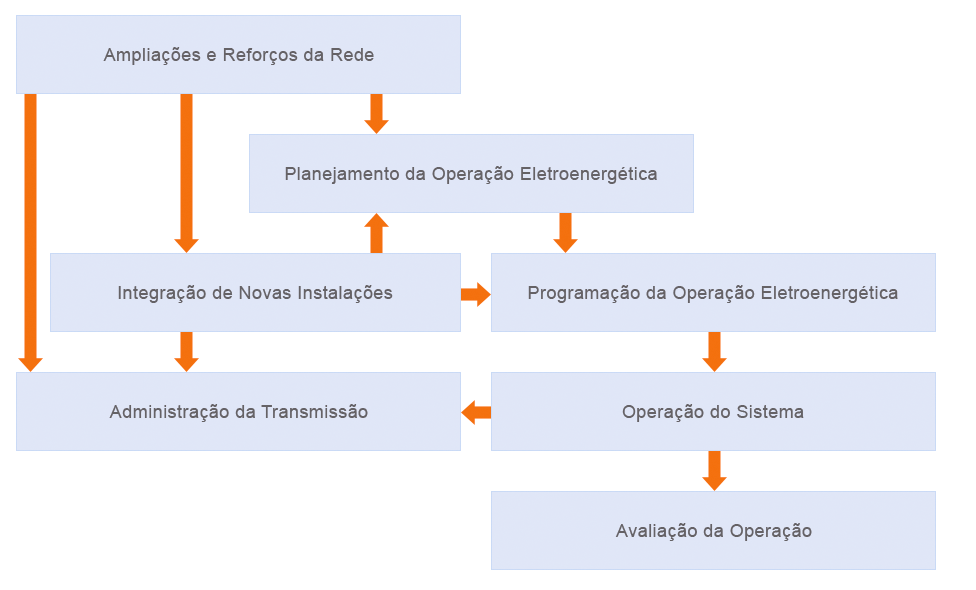
\includegraphics[width=0.5\textwidth]{Figuras/ONS_ABRANGENCIA.png}
\centering
\caption{Área de Atuação da ONS perante o Sistema.}
\label{figura: ONS_AREA}
\end{figure}

\newpage

Já quem faz a operação do sistema nacional é o operador naciona do sistema elétrico (ONS), qual faz desde o planejamento elétrico até operação do sistema como um todo, como mostrada na Figura \ref{figura: ONS_AREA}, a abrangência da ONS perante o SIN.

\subitem{Níveis Hierárquicos}

A análise de confiabilidade pode abranger três níveis
hierárquicos, conforme apresentado na Figura \ref{figura: Niveis_Hierarquicos} \cite{Cassula2003}:
\begin{enumerate}
	\item Nível Hierárquico 0 (NH0): Abrange o estudo de confiabilidade ligado ao sistema energético isolado aos demais, normalmente se analisa a confiabilidade de projeto e funcionamento;
	\item Nível Hierárquico 1 (NH1): Abrange o estudo de confiabilidade ligado a geração de energia;
	\item Nível Hierárquico 2 (NH2): Abrange o estudo de confiabilidade ligados a transmissão e geração de energia;
	\item Nível Hierárquico 3 (NH3): Abrange o estudo de confiabilidade ligados a distribuição, transmissão e geração de energia.
\end{enumerate}

\begin{figure}[h]
	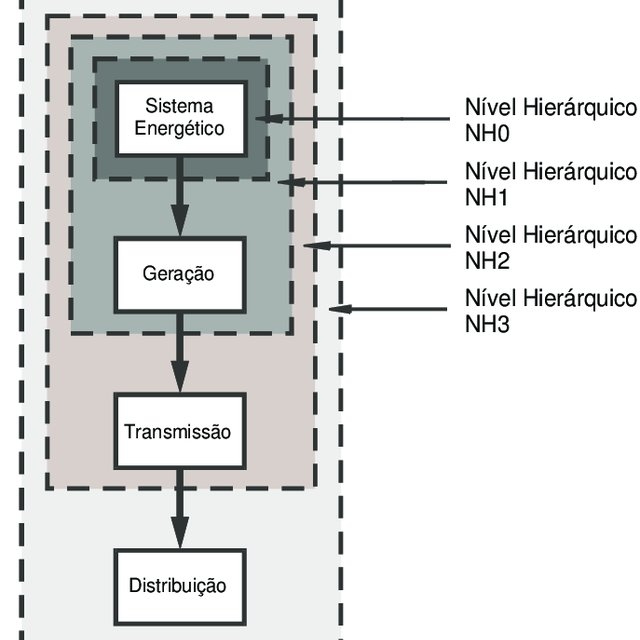
\includegraphics[width=0.3\textwidth]{Figuras/Figura-1-Niveis-Hierarquicos-de-um-Sistema-de-Potencia.jpg}
	\centering
	\caption{Níveis Hierárquicos de um Sistema de Potencia\cite{Cassula2003}.}
	\label{figura: Niveis_Hierarquicos}
\end{figure}

Atualmente devido a dimensão dos problemas trabalhamos apenas com o NH2, assim montando o problema em razão das falhas em linhas de transmissão quais já foram modeladas e levantadas.

\section{Modelagem e Simulações}

Nesta seção apresentam-se as caracteristicas do sistema de transmissão sul brasileiro com 32 barras simulado no \textit{software} ANAREDE, para o cenário proposto para níveis de carregamento e níveis de geração, como um ponto de operação qual haveria contingências se houvesse alguma violação de tensão ou fluxo de potência, assim como considerar contingências os casos divergentes a partir do ponto de operação descrito na Tabela \ref{tabela: Nivel_Carregamento}.

\newcolumntype{Y}{>{\centering\arraybackslash}X}
\begin{table}[ht]
	\caption{Configuração do Nível de Carregamento(MW)}
	\label{tabela: Nivel_Carregamento}
	\centering
	\begin{tabularx}{.4\textwidth}{| Y | Y | Y |}
		\hline
		\multicolumn{3}{|c|}{Nível de Carregamento (MW)} \\
		\hline
		Área 1 & Área 2 & Área 3 \\
		\hline
		3100 & 7800 & -4500 \\
		\hline
	\end{tabularx}
\end{table}

Assim como o nível de carregamento foi definido em cada área do sistema, o nível de geração também foi previamente definido conforme a Tabela \ref{tabela: Nivel_Geracao}.

\begin{table}[ht]
	\caption{Configuração do Nível de Carregamento(MW)}
	\label{tabela: Nivel_Geracao}
	\centering
	\begin{tabularx}{.4\textwidth}{| Y | Y |}
		\hline
		\multicolumn{2}{|c|}{Nível de Geração } \\
		\hline
		Área 1 & Área 2 \\
		\hline
		-20\% & -20\% \\
		\hline
	\end{tabularx}
\end{table}

Com a definição das tabelas \ref{tabela: Nivel_Carregamento} e \ref{tabela: Nivel_Geracao}, pode-se utilizar o ANAREDE para configuração do sistema conforme as tabela, após carregamento do projeto e configuração das opções das tabelas, o esquemático do sistema STSB-32 foi disposto na Figura \ref{figura: Sistema_STSB_32}, qual mostra os esquemático completo no ANAREDE.

\begin{figure}[h]
	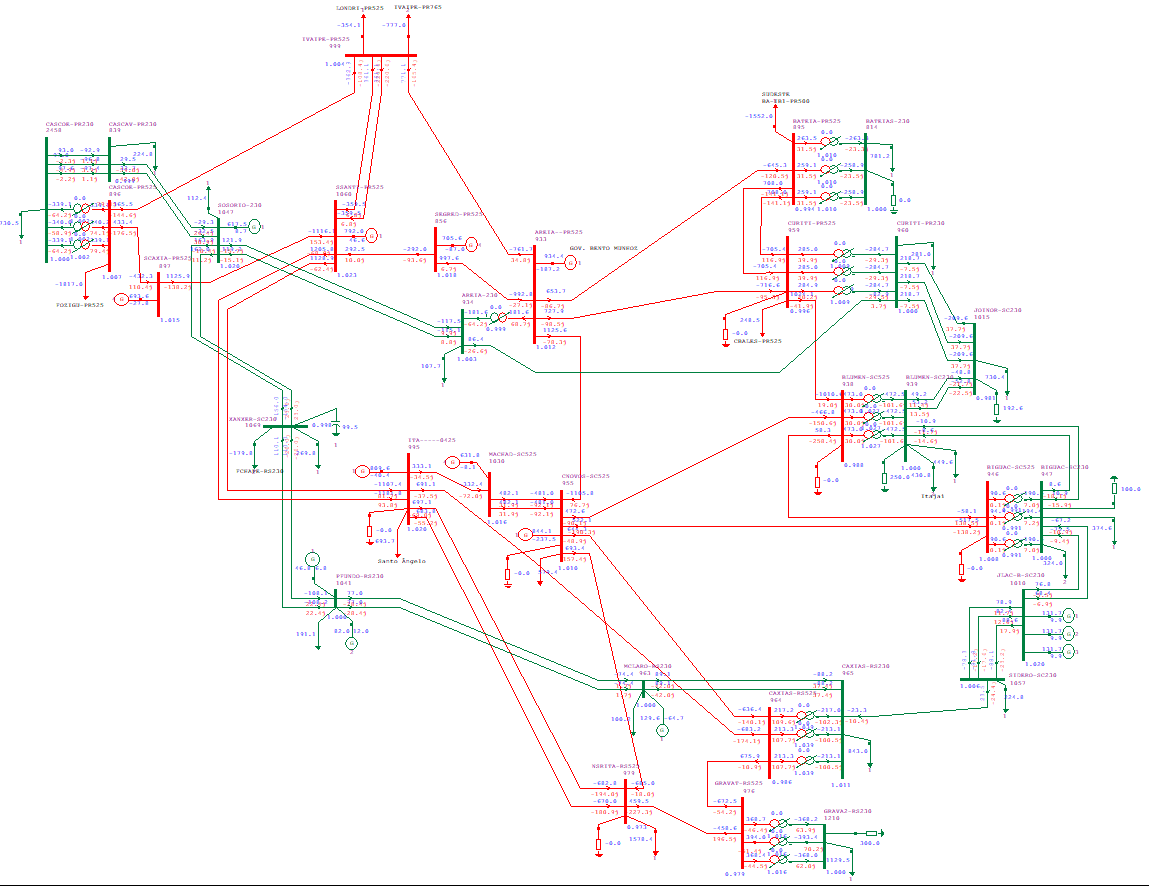
\includegraphics[width=0.5\textwidth]{Figuras/STSB-32.png}
	\centering
	\caption{Diagrama do sistema de transmissão sul brasileiro de 32 barras.}
	\label{figura: Sistema_STSB_32}
\end{figure}

Sendo o sistema separado por tensão, os níveis de tensão são de 230 kV, na cor verde e 525 kV na cor vermelha, esse sistema também é dividido em três áreas. A área número 1 é a parte classificada em 525 kV, a área 2 é a parte do sistema em 230 kV e a área 3 é a área de importação de energia da região sudeste do Brasil.



\section{Other Resources}
See for resources on formatting math into text and additional help in working with \LaTeX .

\section{Text}



\section{Some Common Elements}

\subsection{Arrays}



\section{Conclusion}
The conclusion goes here.


%{\appendices
%\section*{Proof of the First Zonklar Equation}
%Appendix one text goes here.
% You can choose not to have a title for an appendix if you want by leaving the argument blank
%\section*{Proof of the Second Zonklar Equation}
%Appendix two text goes here.}
 
\bibliography{LeonardoReferencias}
\bibliographystyle{IEEEtran}

\end{document}



